\documentclass[conference]{IEEEtran}
\IEEEoverridecommandlockouts
% The preceding line is only needed to identify funding in the first footnote. If that is unneeded, please comment it out.

% RULES: 
% The length for final papers is a maximum of 4-6 pages without exceptions.
% Each paper should indicate appropriateness for the conference's scope, originality, quality of the technical content, whole organization, and writing style. The paper should, moreover, explain the significance of the contribution and contain a list of key references.
% A submission implies a willingness to register and present the work if the paper is accepted for presentation at the Conference.
\usepackage{cite}
\usepackage{amsmath,amssymb,amsfonts}
\usepackage{algorithmic}
\usepackage{graphicx}
\usepackage{textcomp}
\usepackage{subcaption}
\usepackage{xcolor}
\usepackage{hyperref}
\usepackage{cleveref}
\def\BibTeX{{\rm B\kern-.05em{\sc i\kern-.025em b}\kern-.08em
    T\kern-.1667em\lower.7ex\hbox{E}\kern-.125emX}}
\begin{document}

\title{Real-Time Detection of Passive MRI Guidewire for Endovascular Intervention}

\author{\IEEEauthorblockN{1\textsuperscript{st} Martin Reinok}
\IEEEauthorblockA{\textit{Embedded Systems ??} \\
\textit{University of Twente}\\
Enschede, Netherlands \\
m.reinok@student.utwente.nl}
\and
\IEEEauthorblockN{2\textsuperscript{nd} Giulio Dagnino}
\IEEEauthorblockA{\textit{dept. name of organization (of Aff.)} \\
\textit{University of Twente}\\
Enschede, Netherlands \\
g.dagnino@utwente.nl}
\and
\IEEEauthorblockN{3\textsuperscript{rd} Wyger Brink}
\IEEEauthorblockA{\textit{dept. name of organization (of Aff.)} \\
\textit{University of Twente}\\
Enschede, Netherlands \\
w.m.brink@utwente.nl}
}

\maketitle

\begin{abstract}
Vascular and cardiac interventions often rely on X-ray fluoroscopy for real-time imaging guidance, which poses risks due to ionizing radiation exposure. Magnetic resonance imaging (MRI) offers a safer alternative with superior soft tissue contrast, but its adoption for real-time guidance has been limited by technical challenges. This paper presents a novel approach for real-time detection of passive MRI guidewires during endovascular interventions, addressing key limitations of MRI guidance. A convolutional neural network (CNN) is trained using a procedurally generated dataset to detect susceptibility artifacts in a MR-safe guidewire. The CNN output is integrated into a software system that provides automatic guidewire tracking and MRI slice alignment, enabling real-time visualization of the scan plane, detected guidewire, and patient anatomy. Experimental results demonstrate the effectiveness of the proposed approach in accurately detecting passive guidewires in a phantom, under varying imaging conditions. The system shows promise in improving the safety, efficiency, and accuracy of MRI-guided interventions.
\end{abstract}

\begin{IEEEkeywords}
MRI-guided interventions, passive guidewire detection, susceptibility artifacts, endovascular intervention, image-guided procedures
\end{IEEEkeywords}

\section{Introduction}
Vascular and cardiac ailments continue to be significant contributors to illness and death rates. X-ray fluoroscopy is widely used form of therapy for this type of diseases. The navigation of endovascular catheters during interventions often requires the use of image guidance. While X-ray is currently the preferred modality for real-time imaging due to its commendable spatial and temporal resolution, it has notable drawbacks including exposure to ionizing radiation for patients and medical personnel, and limited soft tissue characterization.

Magnetic resonance imaging (MRI) has been introduced as a promising alternative. Both clinical and experimental studies conducted using MR fluoroscopy have demonstrated its effectiveness in various procedures, including the delivery of ASD closure, aortic valves, and endovascular stents (such as those used in the aortic, carotid, iliac, renal arteries, and inferior vena cava) \cite{pmid21359519}. Contrary to fluoroscopy, MRI provides high soft-tissue contrast, three-dimensional data and avoids exposure to ionizing radiation. 

However despite the benefits, MRI has it's shortcomings, which have suppressed it from becoming the preferred modality for procedures. Most notably, the following issues have been highlighted to be significant from clinical trials \cite{pmid35420239}:
\begin{itemize}
    \item Low temporal/spatial resolution
    \item Guidewire/catheter visibility
    \item Safety (device visibility)
    \item Manual MRI slice alignment
\end{itemize}
MRI in general must balance a tradeoff between resolution, signal-to-noise ratio (SNR) and repetition time (TR). Even though the spatial resolution can be increased very high, resulting in image quality that even surpasses x-ray, the repetition time will increase and therefore also real-time capabilities will drop significantly. Introduction of sliding window technique allowed MRI to reach real-time frame rates, up to 30 Hz \cite{pmid3173063}. While this is close to on-par with X-ray, the temporal/spatial resolution of such sequences is not great. In this study, real-time target of 3 Hz imaging is focused, which provides sufficient spatial/temporal resolution, with reasonable latency. 

To counter the device visibility issues, there are primarily two options produced by companies: active and passive. Active devices have improved visibility, but introduce additional complexity and may pose safety concerns, whereas passive devices do not require external power sources and rely on the embedding of magnetic nanoparticles for visibility. In this study, we focus exclusively on passive devices. There are many commercial options for passive devices, some examples include MaRVis\cite{marvistech-guidewires}, Nano4Imaging\cite{nano4imaging-guidewires} and EPflex \cite{epflex-guidewires}, all using markers caused by \(B_0\) field inhomogeneities, to enhance the visibility during MRI scans.
% \textbf{TODO: What has been done in literature to fix these problems}

Here we propose a work-in-progress design of a software integration layer for a MRI system, which is capable of detecting MR-safe passive endovascular guidewire from real-time (interactive) equivalent MR sequences. The detection is achieved by using a Convolutional Neural Network (CNN), using a procedural-generated dataset, to avoid manual annotation and MR imaging. The software provides detection, an ad-hoc guidewire tracking algorithm, automatic slice alignment to track the passive guidewire, and future possibility for 3D visualization of the scan plane and detected guidewire relative to the patient.

The proposed software aims to provide a comprehensive solution for MR-guided interventions, by improving the safety, efficiency, and accuracy.
% \textbf{TODO: What we propose and how does it help}

\section{Methods}

\subsection{TODO: MRI settings}\label{MRI-settings}

\begin{itemize}
    \item bSSFP
    \item Voxel size: 1.2 - 1.4
    \item TR: 470 ms
    \item TE: 1.5 ms
    \item 256 matrix
    \item 
\end{itemize}
Comparison of GRE + bSSFP + slice thickness.
A series of experiments was designed to optimize marker visibility and detection.
Settings, explanations, fine-tuning.

\subsection{Susceptibility Artifact Simulation}\label{artifact-simulation}
The endovascular devices used for fluoroscopy are commonly made of nitinol (nickel-titanium), a material that does not create a signal under MRI, and is not visible. To combat this, the devices have been incorporated with paramagnetic markers, usually made of gadolinium or iron. These markers create localized distortions, known as susceptibility artifacts, under MRI and make the guidewire partially visible. \autoref{fig:xray-vs-mri-guidewire-comparison} demonstrates the difference between X-ray and MRI device visibility. 

\begin{figure}[h]
    \centering
    \begin{minipage}{0.241\textwidth}
        \centering
        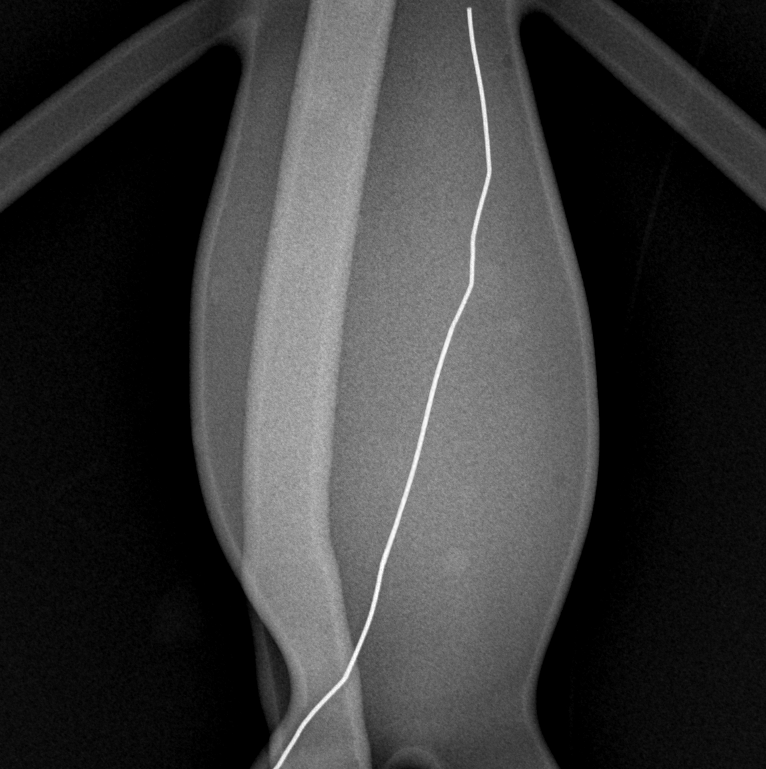
\includegraphics[width=\textwidth]{Conference/img/xray-device-visibility.png}
        \subcaption*{(a)}
    \end{minipage}\hfill \hspace*{0cm}
    \begin{minipage}{0.241\textwidth}
        \centering
        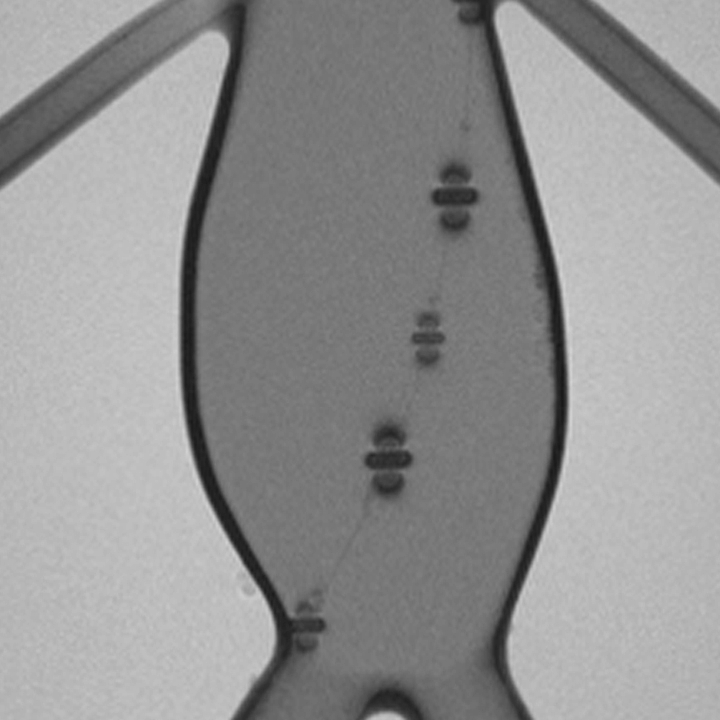
\includegraphics[width=\textwidth]{Conference/img/mri-device-visibility.jpg}
        \subcaption*{(b)}
    \end{minipage}\hfill \hspace*{0cm}
    \caption{Comparison of endovascular device visibility under x-ray(a) and MR (b).}
    \label{fig:xray-vs-mri-guidewire-comparison}
\end{figure}

Active tracking is also an option for MR tracking, which employ electronics and RF coils in the tip of the guidewire, which makes it stand out in the image. Their long-term usage is limited due to the fact that it involves electrical leads and might raise safety concerns \cite{pmid11146480}. Passive  tracking,  on  the  other  hand,  yields  acquisition-dependent  results  and  does  not generally  offer  adequate spatial-temporal resolution \cite{pmid11146480}.

The guidewire used in this paper, and demonstrated in \autoref{fig:xray-vs-mri-guidewire-comparison} (b) is EPflex MRline, a guidewire designed for MR interventions \cite{epflex-guidewires}.

The embedded paramagnetic markers in passive guidewires create small local magnetic distortion artifacts, which are mathematically well defined. The in-homogeneous part of the field distortion outside the particle is described by a dipole, as given by \cite{pmid14523965}:

\begin{equation}
\label{eq:dipole-field-distortion}
B_z = c \cdot \frac{(x^2 + y^2 - 2z^2)}{(x^2 + y^2 + z^2)^{\frac{5}{2}}}\text{, where } c = \frac{B_0 \cdot \Delta{\chi} V}{4 \pi}
\end{equation}

Here, \(B_0\)(T) is the main magnetic field, \(\Delta{\chi}\) is the susceptibility difference between the marker material and the surrounding tissues, and \(V\) is the volume of the paramagnetic material. \(x\), \(y\) and \(z\) represent the spatial coordinates.

The simulation of \eqref{eq:dipole-field-distortion} is shown in \autoref{fig:simulations}(a). To simulate the signal of the coronal magnitude of a realistic artifact, integration over the slice thickness is necessary \cite{pmid14523965}:

\begin{equation}
\label{eq:integration-over-slice-formula}
S_{coronal} = \int_{-d/2}^{d/2} {\rho}(x,y,z) \exp(-i\gamma B_z TE) \,dz
\end{equation}

Here, \(\rho (x,y,z)\) is the signal producing spin density. Assuming uniform spin density, \(\rho (x,y,z)\) is taken as 1. \(d\) is the slice thickness, \(\gamma\) (Hz/T) is gyromagnetic ratio and \(TE\) the echo time. Simulation of \eqref{eq:integration-over-slice-formula} results in \autoref{fig:simulations}(b).

\begin{figure}[h]
    \centering
    \begin{minipage}{0.241\textwidth}
        \centering
        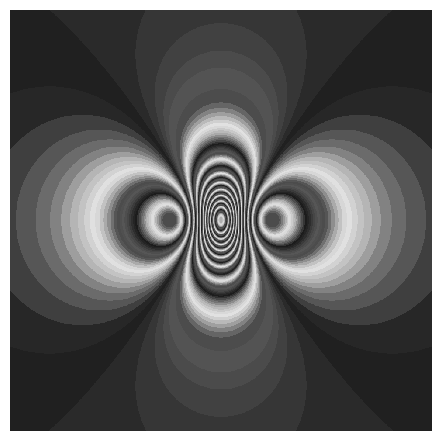
\includegraphics[width=\textwidth, angle=90]{Conference/img/dipole-field-distortion.png}
        \subcaption*{(a)}
    \end{minipage}\hfill \hspace*{0cm}
    \begin{minipage}{0.241\textwidth}
        \centering
        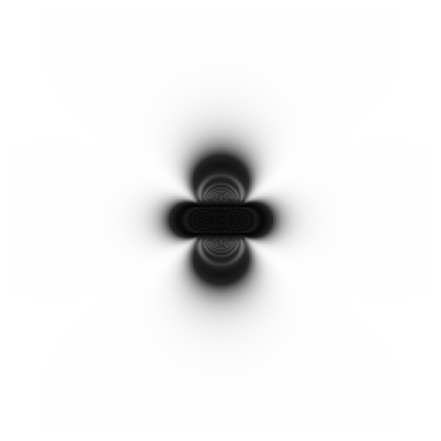
\includegraphics[width=\textwidth]{Conference/img/coronal-magnitude-simulation.png}
        \subcaption*{(b)}
    \end{minipage}\hfill \hspace*{0cm}
    \caption{(a) Dipole Field Distortion,
    (b) Simulated Coronal Magnitude.}
    \label{fig:simulations}
\end{figure}

\subsection{Procedural Artifact Dataset for CNN}\label{artifact-cnn-dataset}
To avoid manual annotation of susceptibility artifacts, and also having to take many images with the MRI, an alternative procedural method is presented. The generated susceptibility artifact is first masked by it's signal value, resulting in a segmentation truth mask. The generated artifact is then superimposed on existing MRI images. The scale, contrast and the number of artifacts on image are augmented withing a reasonable range, increasing variability, detection under multiple slice thicknesses and the overall CNN robustness.

A dataset of 26 background images was used, which included images of aneurysm phantom, images of heart from online dataset and plain background images with variable noise and resolution. A region of interest was chosen for each image, to limit the placement range of artifacts (\autoref{fig:background-dataset}). The placement of artifacts was further restricted to be a minimum distance from other already placed markers. That is to avoid overlapping, which is not feasible in real tests.

% \textbf{TODO: MRI Sequence Settings!}

\begin{figure}
    \centering
    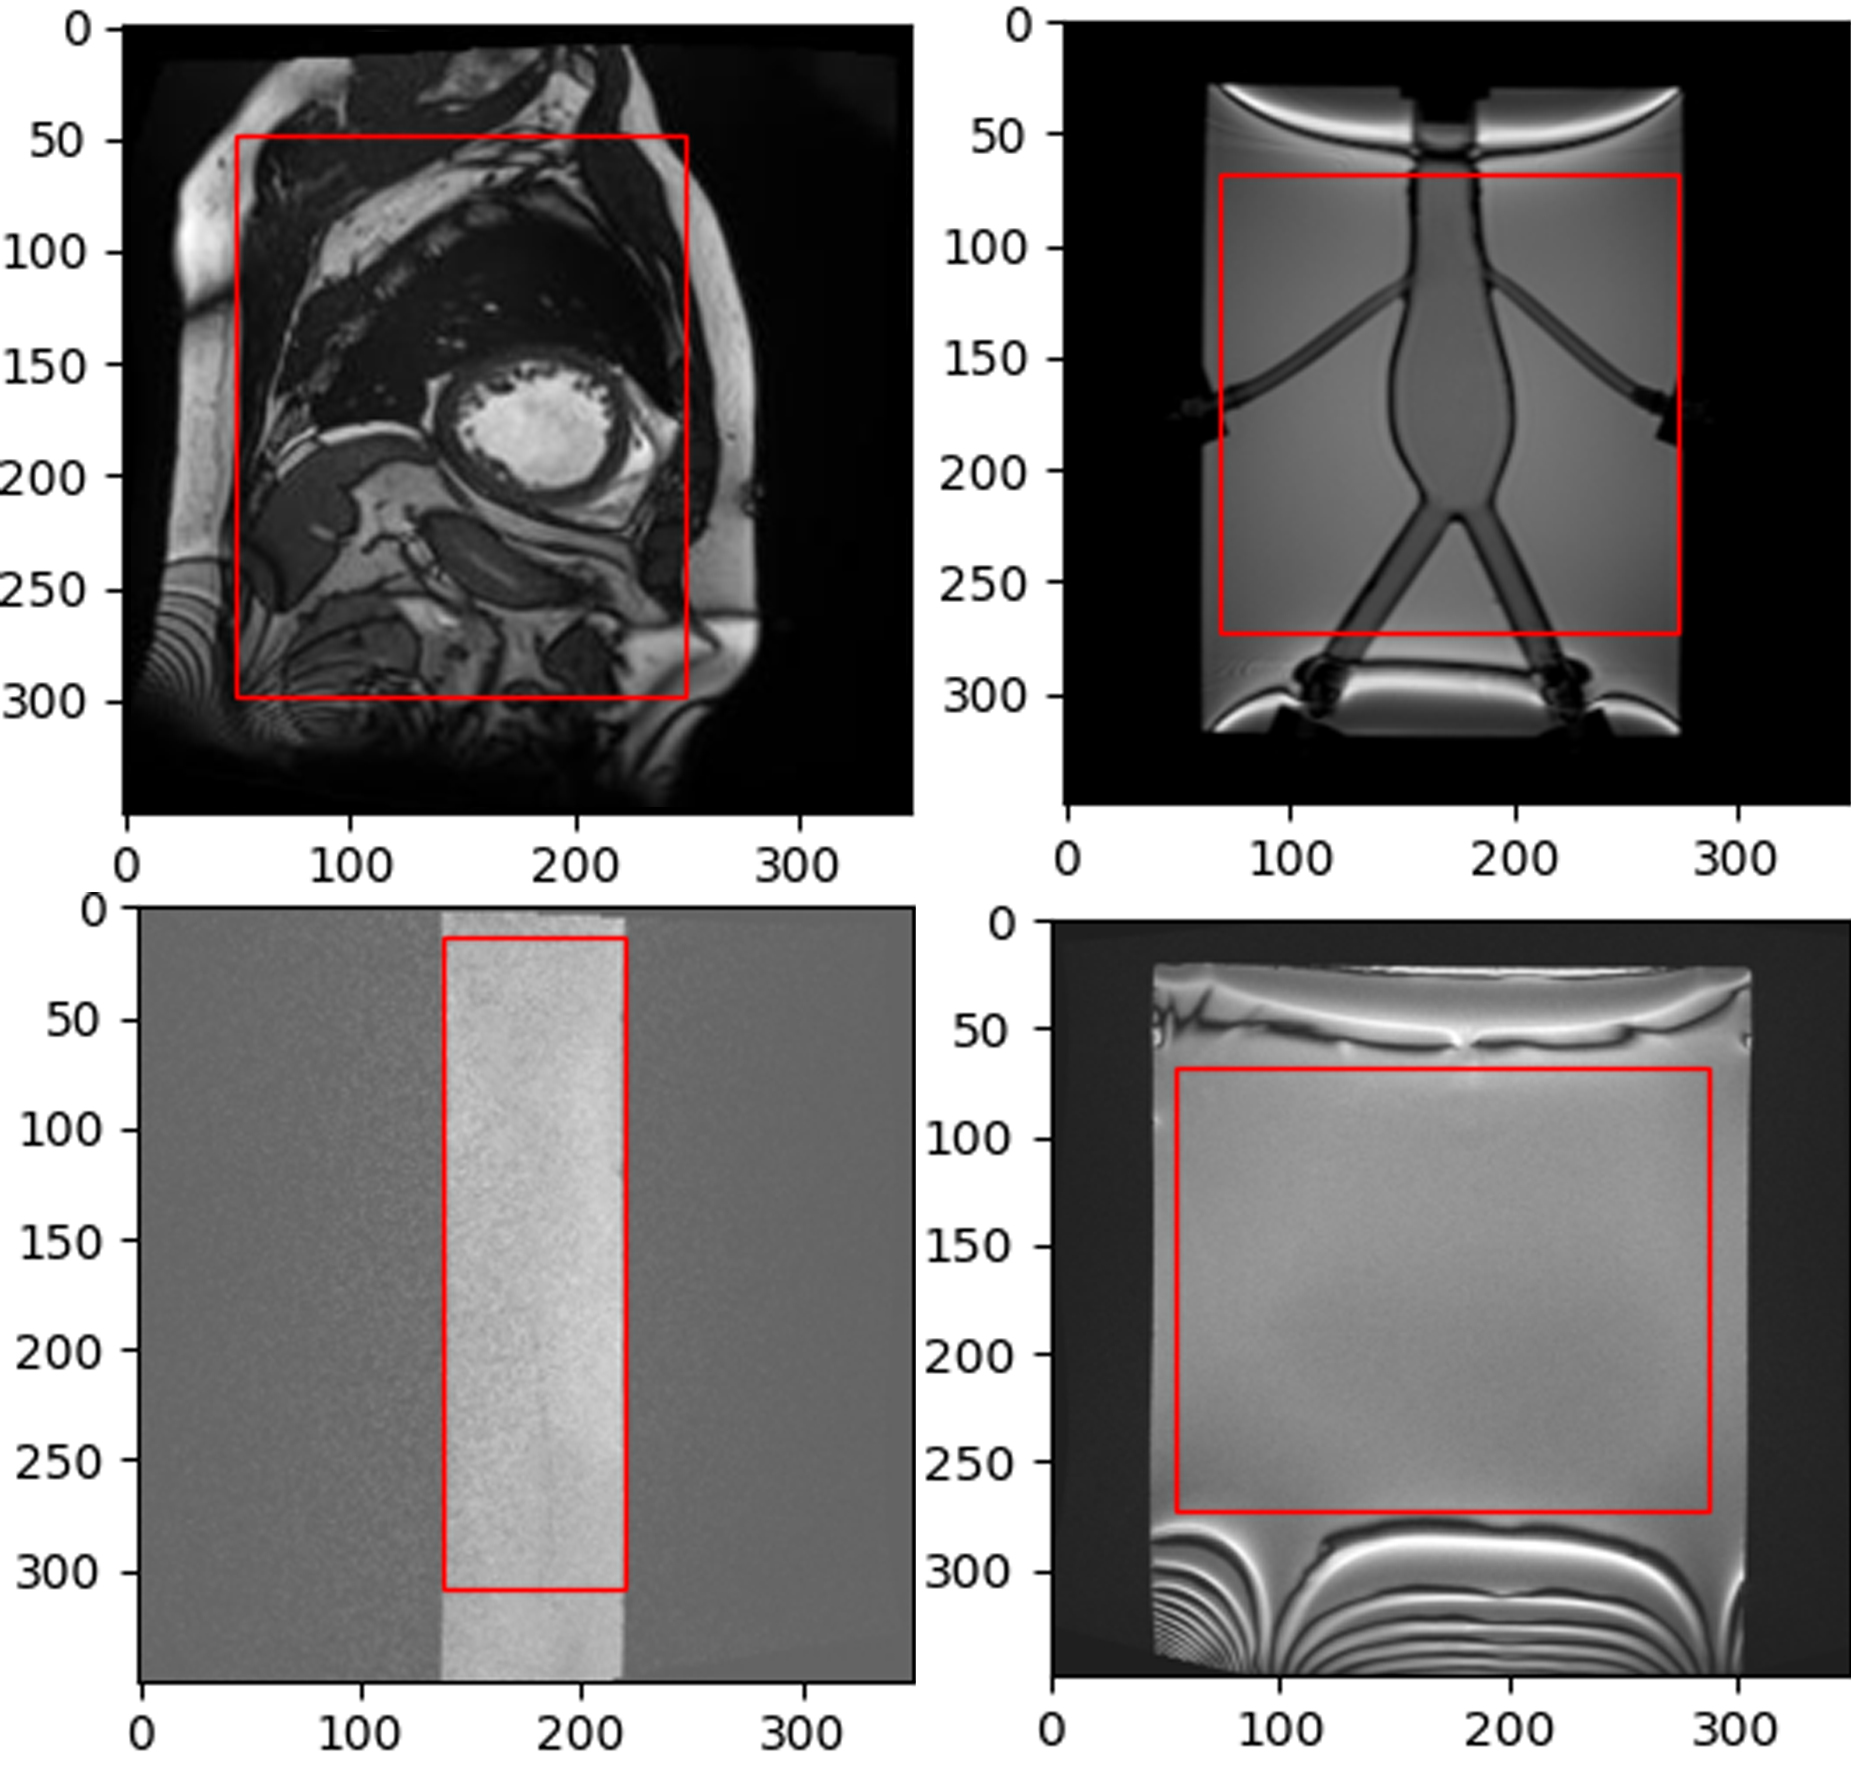
\includegraphics[width=1\linewidth]{Conference//img/roi-example-background-dataset.png}
    \caption{Example of background dataset with a red box, where markers can be procedurally placed (Heart dataset \cite{pmid29994302}).}
    \label{fig:background-dataset}
\end{figure}


\begin{figure}[h]
    \centering
    \begin{minipage}{0.241\textwidth}
        \centering
        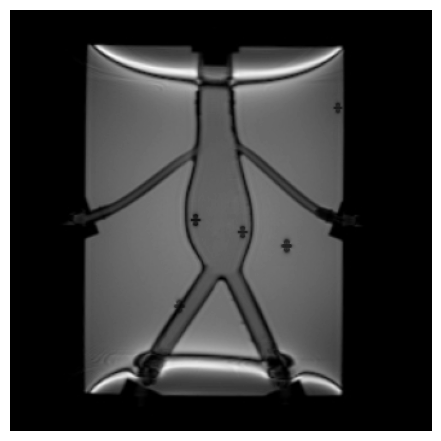
\includegraphics[width=\textwidth]{Conference/img/generated-image.png}
        \subcaption*{(a)}
    \end{minipage}\hfill \hspace*{0cm}
    \begin{minipage}{0.241\textwidth}
        \centering
        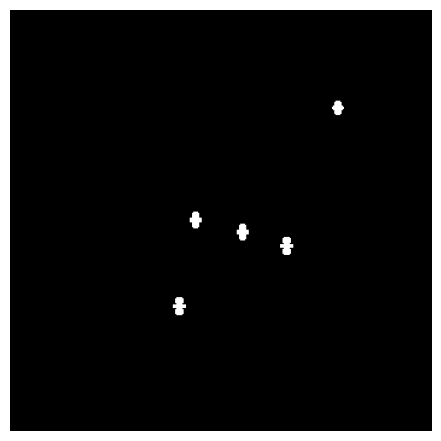
\includegraphics[width=\textwidth]{Conference/img/generated-image-truth.png}
        \subcaption*{(b)}
    \end{minipage}\hfill \hspace*{0cm}
    \caption{(a) Procedurally generated dataset image,
    (b) Matching CNN truth mask.}
    \label{fig:generated-dataset-and-truth}
\end{figure}

\subsection{Training CNN}\label{training-cnn}
For training the CNN to detect susceptibility artifacts, we utilized the nnUNet framework, which provides a robust infrastructure for medical image segmentation tasks. The training process was conducted using the following specifications (configured automatically by nnUNet):

\begin{itemize}
    \item \textbf{Features}: 32.
    \item \textbf{Convolutions}: 2, for both encoder and decoder.
    \item \textbf{Kernel Sizes}: Pooling: \(2 \times 2\), and convolutional layers: \(3 \times 3\).
    \item \textbf{Image size}: (upsampled) 512x512px
\end{itemize}

\subsection{Guidewire Tracking}\label{guidewire-tracking}
In MRI-guided interventions, real-time tracking of the passive guidewire is essential for accurate device navigation, as well as automatic MRI slice movement to guidewire. However, there are many inherent challenges posed by the described MRI and CNN combination:
\begin{itemize}
    \item Guidewire can enter and exit MRI slice. (visibility)
    \item Low signal-to-noise ratio (SNR) can negatively impact CNN with very fast repetition time sequences.
    \item CNN can have false positives.
    \item Flow artifacts caused by guidewire- and blood movement impact susceptibility artifact visibility (blurring, ghosting, loss of SNR).
\end{itemize}

To address these challenges, an ad-hoc tracking algorithm was developed, tailored for separating and tracking the movement of guidewire from potentially noisy and unpredictable CNN output. The algorithm operates in conjunction with the CNN and is capable of moving the MRI plane in two axis, to match the movement of guidewire.

The algorithm takes the binary image from CNN output as input and applies median blur with threshold to remove any noise and low-probability detections. This will remove the majority of false positives, which are usually salt-style noise. The remaining blobs are considered to be susceptibility artifacts and are continuously tracked. There could still be false positives, as any paramagnetic sphere-like object will create a susceptibility artifact similar to those of the guidewire. For instance metallic fixation screws in the tibia, which create nearly identical susceptibility artifacts \cite{pmid22162977}. However, those false positives should stay in one position, as opposed to the guidewire which is in movement. The algorithm takes this into account to further separate guidewire from the rest.

To track the artifacts, an approach is used which combines Euclidean distance-based matching with linear trajectory prediction. The algorithm maintains a list of active trackers, each associated with a detected artifact. In each frame, each tracker updates it's position based on the detected artifacts in that frame. If associated artifact is not found within specified euclidean distance for more than a predefined threshold of frames, it is considered lost and removed from the list of active trackers.

To estimate and predict the movement of guidewire, each tracker has a initial position and a updated latest position for each frame. The difference of each initial and updated position from the trackers is averaged, while differences of insignificant amount are not considered (e.g. fixation screws). This results in a movement vector which can be predicted linearly for the next frame. Using the movement vector, either predicted or not, the MRI slice can be moved, to motion track the guidewire. 

\section{Results}

\subsection{Artifact Simulation}

Constants similar to our real MRI sequence were initialized. The field-of-view (FOV) was chosen smaller to preserve more quality, which was later down scaled to match actual artifact size.
\begin{itemize} 
    \item \(B_0\): 1.5 T
    \item \(\Delta{\chi} V\): 0.012
    \item \(Echo Time (TE)\): 4.45 ms
    \item \(\gamma\): 42576384.7 Hz/T
    \item \(d\): 10 mm
\end{itemize}

The spatial range for simulation was initialized using a 3D meshgrid, size defined by FOV. The dipole field (\ref{eq:dipole-field-distortion}) is calculated for each element and the integration (\ref{eq:integration-over-slice-formula}) is performed using the dipole field. A custom linear gray-scale colormap is applied on the resulting simulation, to get the output shown in \autoref{fig:simulations}. The superimposed simulations are compared with real artifacts in figure \autoref{fig:real-artifact-vs-simulated-comparison}.

\begin{figure}[h]
    \centering
    \begin{minipage}{0.241\textwidth}
        \centering
        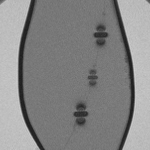
\includegraphics[width=\textwidth]{Conference/img/artifact-real.jpg}
        \subcaption*{(a)}
    \end{minipage}\hfill \hspace*{0cm}
    \begin{minipage}{0.241\textwidth}
        \centering
        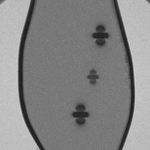
\includegraphics[width=\textwidth]{Conference/img/artifact-generated-superimposed.jpg}
        \subcaption*{(b)}
    \end{minipage}\hfill \hspace*{0cm}
    \caption{(a) Real Artifacts
    (b) Superimposed Simulated Artifacts}
    \label{fig:real-artifact-vs-simulated-comparison}
\end{figure}

\subsection{CNN}

Using the procedural dataset generation described in \ref{artifact-cnn-dataset}, approximately 1000 images were generated to train the CNN.

Using the nnUNet architecture, the standard five cross-validation folds training was done, where the best performing fold was selected for inference and real-time prediction. The dataset was split 80-20 percent, where randomized 20 percent was used for validation at the end of each fold.

The training model was trained until approximate convergence, at 100 epoch. Training achieved pseudo-DICE score of: 0.9957, and best Mean Validation Dice: 0.9974.

The real-time inference latency for the prediction was around 0.3 seconds on a NVIDIA RTX 3090 GPU. This time significantly increased when using slower GPUs. 

Accuracy during real-time inference can be described as sufficient. Most of the time, all fully-visible artifacts were detected. During rapid guidewire movement, disturbance caused by flow artifacts resulted in some detection gaps for 1-2 frames (\autoref{fig:flow-artifacts-tracking}). False positives that can not be filtered out (e.g. fixation screws discussed in \ref{guidewire-tracking}) were to be expected and were also detected by the CNN.

\subsection{Tracking and Slice alignment}
Tracking slow guidewire movement was stable and accurate. As the guidewire speed increases, the flow artifacts become increasingly destructive due to flow artifacts, causing the tracking to lose context and re-initialize once the guidewire has slowed down enough. An example of flow artifacts is shown in \autoref{fig:flow-artifacts-tracking}.

\begin{figure}[h]
    \centering
    \begin{minipage}{0.241\textwidth}
        \centering
        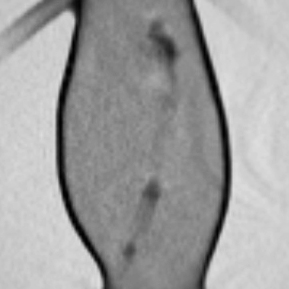
\includegraphics[width=\textwidth]{Conference/img/flow-artifact-with.jpg}
        \subcaption*{(a)}
    \end{minipage}\hfill \hspace*{0cm}
    \begin{minipage}{0.241\textwidth}
        \centering
        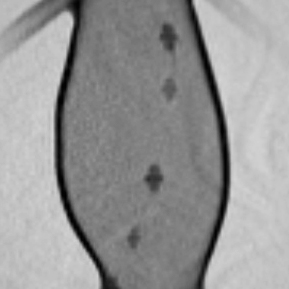
\includegraphics[width=\textwidth]{Conference/img/flow-artifact-without.jpg}
        \subcaption*{(b)}
    \end{minipage}\hfill \hspace*{0cm}
    \caption{(a) Flow artifacts when moving guidewire very fast
    (b) Flow artifacts disappear a second or so after movement}
    \label{fig:flow-artifacts-tracking}
\end{figure}

Tracking itself can not easily be quantified, as the accuracy is heavily dependent of the CNN. The center coordinates of each tracker is chosen to be the centroid of the detected artifact. That means, due to the slight inconsistencies of the CNN, the center coordinates can vary within the confines of the detected artifact, translating to ~$\pm$5 mm of possible fluctuation in artifact position in MRI reference axis. The fluctuation only applies to uncertain, low SNR or high noise detections. Slice alignment accuracy is likely higher, as all trackers are considered for movement calculations.

\begin{figure}[htbp]
    \centering
    \begin{minipage}[t]{0.49\textwidth}
        \centering
        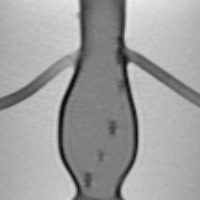
\includegraphics[width=0.49\linewidth]{Conference/img/tracking-websocket-start.jpg}
        \vspace{0.1cm}
        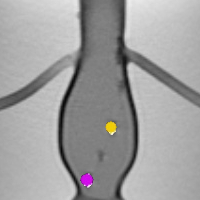
\includegraphics[width=0.49\linewidth]{Conference/img/tracking-websocket-tracks-start.jpg}
    \end{minipage}
    \begin{minipage}[t]{0.49\textwidth}
        \centering
        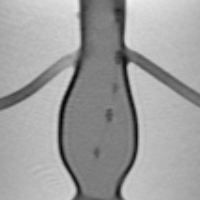
\includegraphics[width=0.49\linewidth]{Conference/img/tracking-websocket-end.jpg}
        \vspace{0.1cm}      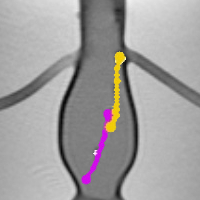
\includegraphics[width=0.49\linewidth]{Conference/img/tracking-websocket-tracks-end.jpg}
    \end{minipage}
    \caption{Guidewire tracking progress. Limited to 2 trackers for visualization purposes.}
    \label{fig:tracking-algorithm}
\end{figure}


\section{Discussion}

\subsection{Summary of findings}
Susceptibility artifact simulation was surprisingly accurate and flexible. Although the accuracy could be further improved by implementing more complex formulas for balanced Steady State Free Precession (bSSFP) as discussed in \cite{sunil-patil-phd}, the current simulation is sufficient as the susceptibility artifacts are scaled down drastically and most details are lost.

Using the procedurally generated dataset can be considered a success as it did save time and effort instead of manually annotating and taking images using MRI. It also provides flexibility to train detection on existing datasets, or even specific individual. Due to the unique and uniform shape of the susceptibility artifact, the training was able to achieve a very high mean and DICE accuracy. This accuracy also translated into accurate real-time detection. 

The trained CNN detection under difficult circumstances, e.g. flow artifacts and noisy images could be improved. Under optimal situations with a phantom, the detection was good and once any noise was filtered out it was nearly perfect. 
In-vivo testing has not been done, but it can be expected that the detection accuracy will drop, as anatomy will make detection harder due to lack of contrast between the background and susceptibility artifact.


The ad-hoc tracking algorithm relies on the accuracy of the CNN and works well under optimal situations. The algorithm is also able to handle few difficult edge cases, e.g. artifact disappearance for up to 5 frames and can recover tracking. If the CNN detection is poor, for instance with a very low SNR image, the tracking system is not usable.

\subsection{Results comparison}
Similar work to this project has been done, 
Han Nijsink et al. used manual annotation for marker locations from a trainset of 30 images, with 10 images for validation \cite{pmid35199259}. They achieved similar results, where median number of markers detected from images was equal to the amount of markers in the images. They suggested the use of GRE sequences instead of bSSFP as used here, as GRE does not have passive banding artifacts and is less prone to flow artifacts. However during our testing, GRE sequences could not achieve the same real-time performance as bSSFP. The SNR for bSSFP sequence with a repetition time of 0.5 seconds was significantly better than GRE. However the ability to generate the training dataset procedurally gives the flexibility to switch sequence type quickly.

\subsection{Future work and current limitations}

The project has addressed 3 out of 4 of the concerns raised in the introduction chapter so far. Safety aspect has not been considered yet, but could be improved by additional visualizations, for instance showing where the guidewire might be colliding with a vessel wall. This would require keeping track of the guidewire's movement in three-dimensions, as well as basic anatomy detection, such as 3D mapping vessels.

As the complete software system relies heavily on the CNN, improvements and stabilizing the detection even further would be beneficial. The current system is trained mostly for phantom-based images, a small subset of training data includes anatomical data, and inference on anatomical data has not been concluded. Considering the background anatomy could open up possibilities for in-vivo detection. Additionally, the detection only considers susceptibility artifacts which 
 are parallel with the \(B_0\) orientation. Oblique detection is not considered but could be beneficial. Furthermore, landmark vs segmentation approaches could be compared to find if one is better than other for this purpose.

 The current tracking algorithm is limited to changing MRI slice in only 2 axis (MRI X and Z). (Rotations are not supported by hardware at the moment) and moving in Y direction requires development of a three-dimensional tracking algorithm, which could understand if guidewire is going upwards or downwards from the slice. 

\subsection{Conclusion}
The project outcome is promising so far and greatly reduces the impact of the issues that have been raised regarding MRI for endovascular use. The proposed software is able to detect passive guidewire from real-time MRI sequences and is able to move the MRI slice automatically, eliminating need for manual slice alignment. Guidewire visibility is taken care of by the CNN and the used bSSFP MRI sequences are chosen to have sufficient resolution, while still being responsive enough for real-time feedback, also partly resolving the low resolution issue.


% \section*{Acknowledgment}
\bibliographystyle{vancouver}
\bibliography{references}
\vspace{12pt}

\end{document}
